
\paragraph{GET /:lang/user/:userId/question}
\begin{itemize}
\item \textbf{Successo}
% descrizione diagramma e UML

\textbf{Descrizione}: il \texttt{QuestionRouter} gestisce la richiesta \textit{REST\ped{G}} del Front-End passando il controllo al \texttt{QuestionController}; viene poi invocato il metodo\\ \texttt{getQuestions(req,res,next)} che ritorna tutte le domande create dall'utente.

\begin{figure}[ht]
	\centering
	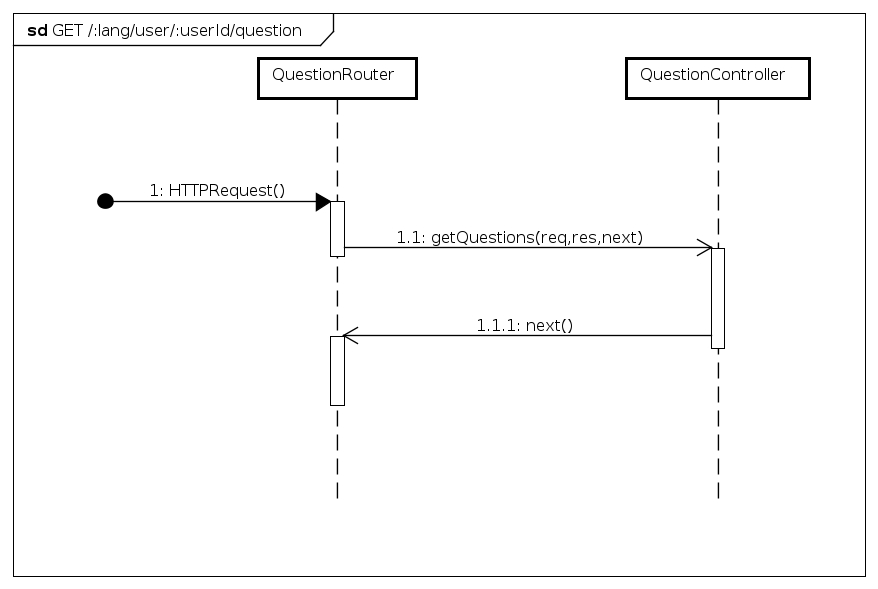
\includegraphics[scale=0.45]{UML/DiagrammiDiSequenza/Back-end/GET__lang_user__userId_question.png}
	\caption{GET /:lang/user/:userId/question}
\end{figure}
\FloatBarrier

\item \textbf{Fallimento}
% descrizione diagramma e UML
\end{itemize}

\paragraph{GET /:lang/user/:userId/question/:questionId}


\paragraph{POST /:lang/user/:userId/question}
\begin{itemize}
\item \textbf{Successo}
% descrizione diagramma e UML

\textbf{Descrizione}: il \texttt{QuestionRouter} gestisce la richiesta \textit{REST\ped{G}} del Front-End passando il controllo al \texttt{QuestionController}; viene poi invocato il metodo\\ \texttt{createQuestion(req,res,next)} che inserisce una nuova domanda creata all'interno del sistema.

\begin{figure}[ht]
	\centering
	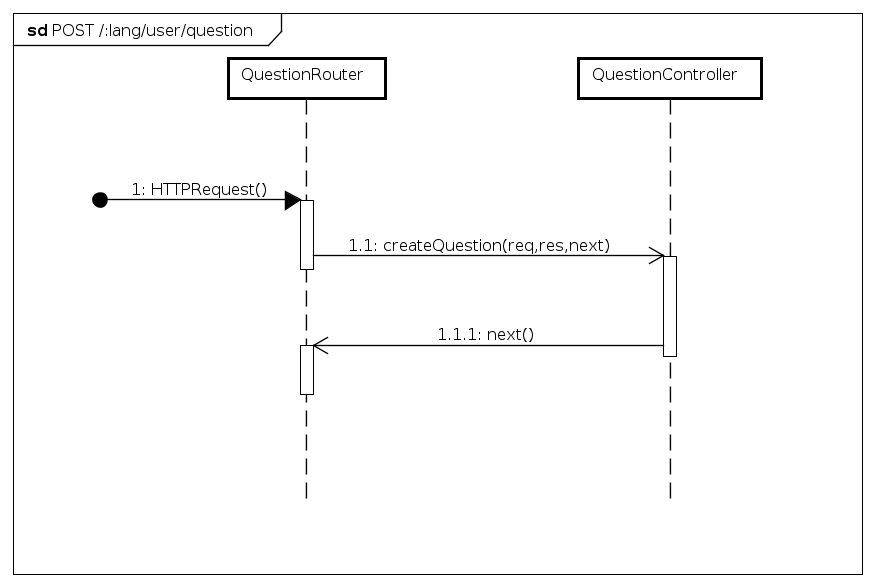
\includegraphics[scale=0.45]{UML/DiagrammiDiSequenza/Back-end/POST__lang_user_question.png}
	\caption{POST /:lang/user/:userId/question}
\end{figure}
\FloatBarrier

\item \textbf{Fallimento}
% descrizione diagramma e UML
\end{itemize}
